\xiti
\begin{xiaotis}

\xiaoti{已知 $\triangle ABD \quandeng \triangle ACE$, $\angle B = \angle C$,指出其他的对应角和对应边;
    又知 $\triangle OBE \quandeng \triangle OCD$,指出所有的对应角和对应边。
}

\begin{figure}[htbp]
    \centering
    \begin{minipage}[b]{4.5cm}
        \centering
        \begin{tikzpicture}
    \tkzDefPoints{0/0/A,  2.5/0/E,  2.5/2.5/C}
    \tkzCalcLength(A,C)    \tkzGetLength{ac}
    \tkzDefPoint(\ac,0){B}
    \tkzInterLC(A,C)(A,E)  \tkzGetSecondPoint{D}
    \tkzInterLL(B,D)(C,E)  \tkzGetPoint{O}

    \tkzDrawPolygon(A,C,E)
    \tkzDrawPolygon(A,B,D)
    \tkzMarkAngles[size=0.3](A,C,E  D,B,A)
    \tkzLabelPoints[below](A,B,E)
    \tkzLabelPoints[right](O)
    \tkzLabelPoints[above](C)
    \tkzLabelPoints[above,xshift=-0.3em](D)
\end{tikzpicture}


        \caption*{(第 1 题)}
    \end{minipage}
    \qquad
    \begin{minipage}[b]{4.5cm}
        \centering
        \begin{tikzpicture}
    \tkzDefPoints{0/0/A,  2.5/0/B,  -0.4/2.5/C, 2.9/2.5/D}
    \tkzInterLL(A,D)(B,C)  \tkzGetPoint{O}

    \tkzDrawPolygon(A,B,C)
    \tkzDrawPolygon(A,B,D)
    \tkzLabelPoints[below](A,B)
    \tkzLabelPoints[above](C,O,D)
\end{tikzpicture}


        \caption*{(第 2 题)}
    \end{minipage}
    \qquad
    \begin{minipage}[b]{4.5cm}
        \centering
        \begin{tikzpicture}
    \tkzDefPoints{0/0/B,  0.6/0/D,  2.4/0/E, 3.0/0/C,  1.5/2.5/A}

    \tkzDrawPolygon(A,B,E)
    \tkzDrawPolygon(A,C,D)
    \tkzMarkAngles[size=0.4](A,E,B  C,D,A)
    \tkzLabelAngle[pos=0.6](A,E,B){$1$}
    \tkzLabelAngle[pos=0.6](C,D,A){$2$}
    \tkzLabelPoints[below](B,D,E,C)
    \tkzLabelPoints[above](A)
\end{tikzpicture}


        \caption*{(第 3 题)}
    \end{minipage}
\end{figure}


\xiaoti{已知 $\triangle ABC \quandeng \triangle BAD$, $BC = AD$,指出其他的对应边和对应角,
    又知 $\triangle OAC \quandeng \triangle OBD$,指出所有的对应边和对应角。
}

\xiaoti{已知 $\triangle ABE \quandeng \triangle ACD$, $\angle 1 = \angle 2$,$\angle B = \angle C$。指出其他的对应边和对应角。}

\xiaoti{画下列三角形:}
\begin{xiaoxiaotis}

    \xxt{腰长等于 $l$, 顶角等于 $\angle \alpha$ 的等腰三角形;}

    \xxt{两条直角边分别等于 $a$ 和 $b$ 的直角三角形。}

\end{xiaoxiaotis}


\xiaoti{在第 1 题的图中,已知:$AB = AC$, $AD = AE$。\\
    求证: $\triangle ABD \quandeng \triangle ACE$。
}

\xiaoti{在第 2 题的图中,已知:$\angle CAB = \angle DBA$, $AC = BD$。\\
    求证: $\triangle CAB \quandeng \triangle DBA$。
}

\xiaoti{已知:点 $A$、$F$、$E$、$C$ 在同一条直线上。 $AF = CE$, $BE \pingxing DF$, $BE = DF$。\\
    求证: $\triangle ABE \quandeng \triangle CDF$。
}


\begin{figure}[htbp]
    \centering
    \begin{minipage}[b]{7cm}
        \centering
        \begin{tikzpicture}
    \tkzDefPoints{0/0/D,  3/0/C,  -1/2/A, 2/2/B}
    \tkzDefPointOnLine[pos=0.4](A,C)  \tkzGetPoint{F}
    \tkzDefPointOnLine[pos=0.4](C,A)  \tkzGetPoint{E}

    \tkzDrawPolygon(A,B,E)
    \tkzDrawPolygon(C,D,F)
    \tkzLabelPoints[left](A,D)
    \tkzLabelPoints[right](B,C)
    \tkzLabelPoints[above](F)
    \tkzLabelPoints[below](E)
\end{tikzpicture}


        \caption*{(第 7 题)}
    \end{minipage}
    \qquad
    \begin{minipage}[b]{7cm}
        \centering
        \begin{tikzpicture}
    \tkzDefPoints{0/0/A,  4/0/B}
    \tkzDefMidPoint(A,B)  \tkzGetPoint{M}
    \tkzDefShiftPoint[M](70:2.5){D}
    \tkzDefShiftPoint[M](110:2.5){C}

    \tkzDrawPolygon(A,M,C)
    \tkzDrawPolygon(B,M,D)
    \tkzMarkAngles[size=0.4](C,M,A  B,M,D)
    \tkzLabelAngle[pos=0.6](C,M,A){$1$}
    \tkzLabelAngle[pos=0.6](B,M,D){$2$}
    \tkzLabelPoints[below](A,M,B)
    \tkzLabelPoints[above](C,D)
\end{tikzpicture}


        \caption*{(第 8 题)}
    \end{minipage}
\end{figure}


\xiaoti{已知:$M$ 是 $AB$ 的中点,$MC = MD$, $\angle 1 = \angle 2$。\\
    求证: $AC = BD$。
}

\xiaoti{如图,可以用两根钢条 $AA'$ 和 $BB'$, 在中点处 $O$ 连在一起做成的工具(卡钳)测量工件内槽的宽。
    按照图写出 “已知” 、 “求证”, 并证明 $AB = A'B'$。
}


\begin{figure}[htbp]
    \centering
    \begin{minipage}[b]{7cm}
        \centering
        \includegraphics[width=5cm]{../pic/czjh1-ch3-xiti7-09.png}
        \caption*{(第 9 题)}
    \end{minipage}
    \qquad
    \begin{minipage}[b]{7cm}
        \centering
        \begin{tikzpicture}
    \tkzDefPoints{0/0/A,  3/0/B,  1/2/D,  4/2/C}
    \tkzInterLL(A,C)(B,D)  \tkzGetPoint{O}

    \tkzDrawPolygon(A,O,B)
    \tkzDrawPolygon(C,O,D)
    \tkzLabelPoints[below](A,B)
    \tkzLabelPoints[above](C,D)
    \tkzLabelPoints[right=0.5em](O)
\end{tikzpicture}


        \caption*{(第 10 题)}
    \end{minipage}
\end{figure}

\xiaoti{已知:$AC$ 和 $BD$ 相交于点 $O$, $OA = OC$, $OB = OD$。 \\
    求证: $DC \pingxing AB$。
}

\xiaoti{在 $\triangle ABC$ 中, $\angle ACB = Rt \angle$,延长 $BC$ 至 $B'$, 使 $CB' = BC$,
    连续 $AB'$, 那么 $\triangle ABB'$ 是等腰三角形。 画出图形,写出已知和求证,并且进行证明。
}

\xiaoti{用刻度尺和量角器画 $\triangle ABC$, 使 $\angle A = 28^\circ$, $\angle B = 33^\circ$, $BC = 4.5\;\limi$。}

\xiaoti{要测量河两岸相对的两点 $A$、$B$ 的距离。 可以在 $AB$ 的垂线 $BF$ 上取两点 $C$、$D$,
    使 $CD = BC$, 再定出 $BF$ 的垂线 $DE$, 使 $A$、$C$、$E$ 在一条直线上,
    这时测得的 $DE$ 的长就是 $AB$ 的长。写出已知和求证,并且进行证明。
}

\begin{figure}[htbp]
    \centering
    \begin{minipage}[b]{7cm}
        \centering
        \includegraphics[width=5cm]{../pic/czjh1-ch3-xiti7-13.png}
        \caption*{(第 13 题)}
    \end{minipage}
    \qquad
    \begin{minipage}[b]{7cm}
        \centering
        \begin{tikzpicture}
    \tkzDefPoints{0/0/A,  2/0/B, 3/0/M}
    \tkzDefPoint(30:3.5){D}
    \tkzDefPoint(-30:3.5){C}

    \tkzDrawSegment(A,M)
    \tkzDrawPolygon(A,B,D)
    \tkzDrawPolygon(A,B,C)
    \tkzMarkAngle[size=0.6](C,A,M)  \tkzLabelAngle[pos=0.9](C,A,M){$1$}
    \tkzMarkAngle[size=0.5](M,A,D) \tkzLabelAngle[pos=0.8](M,A,D){$2$}
    \tkzMarkAngle[size=0.4](C,B,M)  \tkzLabelAngle[pos=0.7](C,B,M){$3$}
    \tkzMarkAngle[size=0.3](M,B,D) \tkzLabelAngle[pos=0.6](M,B,D){$4$}
    \tkzLabelPoints[left](A)
    \tkzLabelPoints[right](C,D)
    \tkzLabelPoints[above left](B)
\end{tikzpicture}


        \caption*{(第 14 题)}
    \end{minipage}
\end{figure}

\xiaoti{已知:如图,$\angle 1 = \angle 2$, $\angle 3 = \angle 4$。\\
    求证 $AC = AD$。
}

\xiaoti{已知:如图,点 $B$、$F$、$C$、$E$ 在同一条直线上, $FB = CE$, $AB \pingxing DE$, $AC \pingxing DF$。\\
    求证: $AB = DE$, $AC = DF$。
}

\begin{figure}[htbp]
    \centering
    \begin{minipage}[b]{7cm}
        \centering
        \begin{tikzpicture}
    \tkzDefPoints{0/0/B,  2/0/C, 1.5/0/F, 3.5/0/E, 1.3/2/A,  2.2/-2/D}

    \tkzDrawPolygon(A,B,C)
    \tkzDrawPolygon(D,E,F)
    \tkzLabelPoints[above](A)
    \tkzLabelPoints[below](B,C,D)
    \tkzLabelPoints[below left](F)
    \tkzLabelPoints[right](E)
\end{tikzpicture}


        \caption*{(第 15 题)}
    \end{minipage}
    \qquad
    \begin{minipage}[b]{7cm}
        \centering
        \begin{tikzpicture}
    \tkzDefPoints{0/0/B,  3/0/C,  1.3/3/A}
    \tkzDefPointOnLine[pos=0.7](A,B)  \tkzGetPoint{D}
    \tkzDefPointBy[translation= from D to A](C)  \tkzGetPoint{F}
    \tkzInterLL(A,C)(D,F)  \tkzGetPoint{E}

    \tkzDrawPolygon(A,B,C)
    \tkzDrawSegments(C,F  D,F)
    \tkzLabelPoints[above](A)
    \tkzLabelPoints[left](B,D)
    \tkzLabelPoints[right](C,F)
    \tkzLabelPoints[above, xshift=0.3em](E)
\end{tikzpicture}


        \caption*{(第 16 题)}
    \end{minipage}
\end{figure}

\xiaoti{已知:如图,$D$ 是 $\triangle ABC$ 的边 $AB$ 上一点, $DF$ 交 $AC$ 于点 $E$, $DE = FE$, $FC \pingxing AB$。 \\
    求证: $AE = CE$。
}

\xiaoti{求证:等腰三角形两腰上的高相等。}

\xiaoti{已知:如图,点 $A$、$B$、$C$、$D$ 在同一条直线上, $AC = BD$, $AM = CN$, $BM = DN$。 \\
    求证: $AM \pingxing CN$, $BM \pingxing DN$。
}

\begin{figure}[htbp]
    \centering
    \begin{minipage}[b]{7cm}
        \centering
        \begin{tikzpicture}
    \tkzDefPoints{0/0/A,  2.5/0/B,  1/0/C, 3.5/0/D, 0.8/2/M,  1.8/2/N}

    \tkzDrawPolygon(A,B,M)
    \tkzDrawPolygon(C,D,N)
    \tkzLabelPoints[above](M,N)
    \tkzLabelPoints[below](A,C,B,D)
\end{tikzpicture}


        \caption*{(第 18 题)}
    \end{minipage}
    \qquad
    \begin{minipage}[b]{7cm}
        \centering
        \begin{tikzpicture}
    \tkzDefPoints{0/0/B,  3.0/0/C,  1.5/3/A,  1.5/0.8/E, 1.5/0/D}

    \tkzDrawPolygon(A,B,C)
    \tkzDrawSegments(A,D  B,E  C,E)
    \tkzLabelPoints[above](A)
    \tkzLabelPoints[below](B,D,C)
    \tkzLabelPoints[right,yshift=0.5em](E)
\end{tikzpicture}


        \caption*{(第 19 题)}
    \end{minipage}
\end{figure}


\xiaoti{已知:如图,$AB = AC$, $EB = EC$, $AE$ 的延长线交 $BC$ 于 $D$。 \\
    求证: $BD = CD$。
}

\xiaoti{已知:$\triangle ABC$ 和 $\triangle DBC$ 的顶点 $A$ 和 $D$ 在 $BC$ 的同旁,$AB = DC$, $AC = DB$, $AC$ 和 $DB$ 相交于点 $O$。 \\
    求证: $OA = OD$。
}

\begin{figure}[htbp]
    \centering
    \begin{minipage}[b]{4.5cm}
        \centering
        \begin{tikzpicture}
    \pgfmathsetmacro{\ab}{1.5}
    \pgfmathsetmacro{\ac}{3.5}
    \tkzDefPoints{0/0/B,  3.5/0/C}
    \tkzInterCC[R](B,\ab)(C,\ac)  \tkzGetFirstPoint{A}
    \tkzInterCC[R](B,\ac)(C,\ab)  \tkzGetFirstPoint{D}
    \tkzInterLL(A,C)(B,D)  \tkzGetPoint{O}

    \tkzDrawPolygon(A,B,C)
    \tkzDrawPolygon(D,C,B)
    \tkzLabelPoints[above](A,O,D)
    \tkzLabelPoints[below](B,C)
\end{tikzpicture}


        \caption*{(第 20 题)}
    \end{minipage}
    \qquad
    \begin{minipage}[b]{4.5cm}
        \centering
        \begin{tikzpicture}
    \pgfmathsetmacro{\ab}{2.5}
    \pgfmathsetmacro{\db}{1.5}
    \tkzDefPoints{0/0/D, 0/1.5/A}
    \tkzInterCC[R](A,\ab)(D,\db)  \tkzGetPoints{C}{B}
    \tkzDefPointOnLine[pos=2.1](A,D)  \tkzGetPoint{E}

    \tkzDrawPolygon(A,B,E,C)
    \tkzDrawSegments(A,E  B,D  C,D)
    \tkzLabelPoints[above](A)
    \tkzLabelPoints[below](E)
    \tkzLabelPoints[left](B)
    \tkzLabelPoints[right](C)
    \tkzLabelPoints[left,yshift=0.3em](D)
\end{tikzpicture}


        \caption*{(第 21 题)}
    \end{minipage}
    \qquad
    \begin{minipage}[b]{4.5cm}
        \centering
        \begin{tikzpicture}
    \tkzDefPoints{0/0/F, 0/3/A, -1.5/2/B, -1/0/C}
    \tkzDefPointBy[reflection = over A--F](B)  \tkzGetPoint{E}
    \tkzDefPointBy[reflection = over A--F](C)  \tkzGetPoint{D}

    \tkzDrawPolygon(A,B,C,D,E)
    \tkzDrawSegments(A,F)
    \tkzLabelPoints[above](A)
    \tkzLabelPoints[below](F)
    \tkzLabelPoints[left](B,C)
    \tkzLabelPoints[right](D,E)
\end{tikzpicture}


        \caption*{(第 22 题)}
    \end{minipage}
\end{figure}

\xiaoti{已知:如图,$AB = AC$, $DB = DC$, $E$ 是 $AD$ 的延长线上一点。 \\
    求证: $BE= CE$。
}

\xiaoti{已知:如图,$AB = AE$, $\angle B = \angle E$, $BC = ED$, $F$ 是 $CD$ 中点。 \\
    求证: $AF \perp CD$。
}

\xiaoti{求证:如果两个三角形有两条边和其中一边上的中线对应相等,那么这两个三角形全等。}

\end{xiaotis}

